\documentclass[tikz,border=4pt]{standalone}
\usepackage[T1]{fontenc}
\usepackage{lmodern}
\usetikzlibrary{arrows.meta,positioning,fit,calc}
\definecolor{indigo}{HTML}{25385C}
\definecolor{teal}{HTML}{176B6A}
\definecolor{lightblue}{HTML}{F1F4FA}
\definecolor{lightteal}{HTML}{EFF7F5}
\definecolor{midgray}{HTML}{5C6570}
\definecolor{lightgray}{HTML}{F5F6F8}
\begin{document}
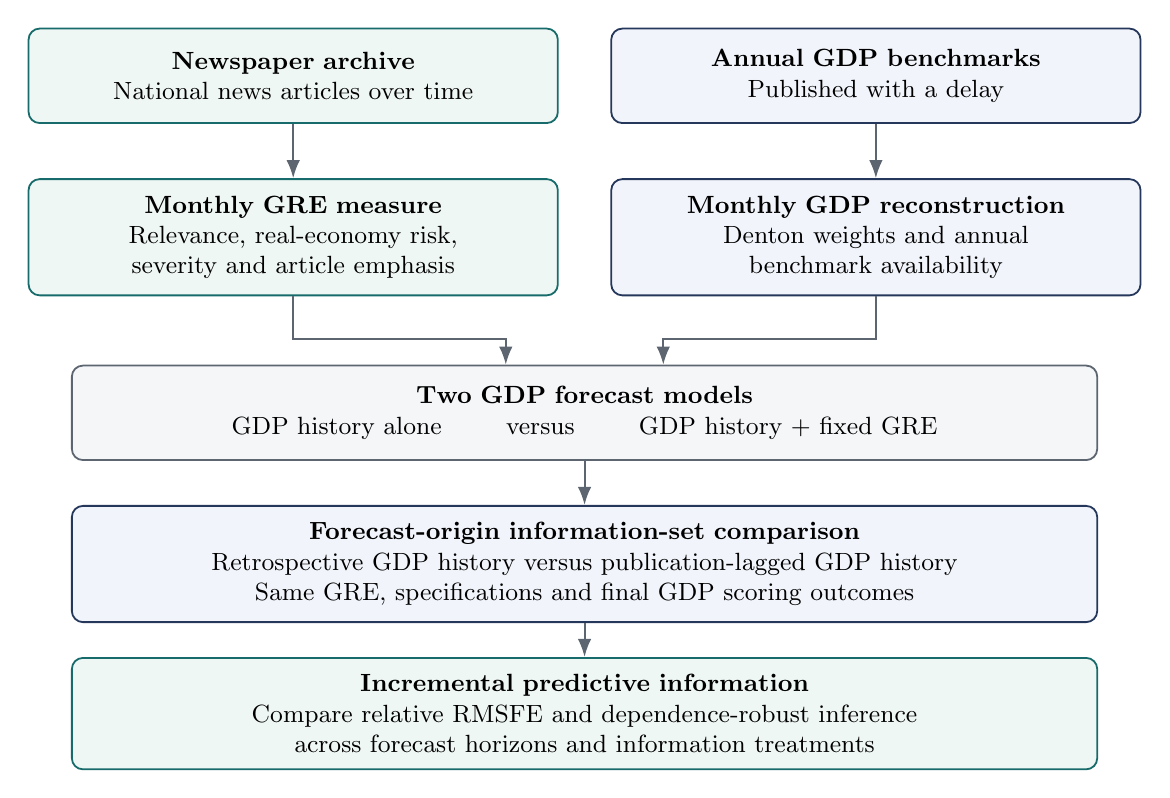
\begin{tikzpicture}[
  font=\sffamily,
  >=Latex,
  base/.style={draw=midgray, line width=.65pt, rounded corners=4pt, align=center, inner sep=6pt, minimum height=12mm, text width=63mm, font=\small},
  risk/.style={base,draw=teal,fill=lightteal},
  gdp/.style={base,draw=indigo,fill=lightblue},
  summarybox/.style={base,draw=midgray,fill=lightgray,text width=126mm,minimum height=12mm},
  arr/.style={-{Latex[length=2.3mm]},line width=.75pt,draw=midgray}
]
\node[risk] (n1) at (-3.7,0) {\textbf{Newspaper archive}\\National news articles over time};
\node[gdp] (g1) at (3.7,0) {\textbf{Annual GDP benchmarks}\\Published with a delay};
\node[risk] (n2) at (-3.7,-2.05) {\textbf{Monthly GRE measure}\\Relevance, real-economy risk,\\severity and article emphasis};
\node[gdp] (g2) at (3.7,-2.05) {\textbf{Monthly GDP reconstruction}\\Denton weights and annual\\benchmark availability};
\draw[arr] (n1)--(n2);
\draw[arr] (g1)--(g2);
\node[summarybox] (j1) at (0,-4.28) {\textbf{Two GDP forecast models}\\GDP history alone \hspace{6mm} versus \hspace{6mm} GDP history + fixed GRE};
\draw[arr] (n2.south) -- ++(0,-0.54) -| ([xshift=-1.0cm]j1.north);
\draw[arr] (g2.south) -- ++(0,-0.54) -| ([xshift=1.0cm]j1.north);
\node[summarybox,draw=indigo,fill=lightblue] (j2) at (0,-6.20) {\textbf{Forecast-origin information-set comparison}\\Retrospective GDP history versus publication-lagged GDP history\\Same GRE, specifications and final GDP scoring outcomes};
\draw[arr] (j1)--(j2);
\node[summarybox,draw=teal,fill=lightteal] (j3) at (0,-8.10) {\textbf{Incremental predictive information}\\Compare relative RMSFE and dependence-robust inference\\across forecast horizons and information treatments};
\draw[arr] (j2)--(j3);
\end{tikzpicture}
\end{document}
